\documentclass{article}
\usepackage[utf8]{inputenc}
\usepackage{amsmath}
\usepackage{amsfonts}
\usepackage{amssymb}

% package for bold math symbols
\usepackage{bm}

% image library + path
\usepackage{graphicx}
\graphicspath{ {./images/} }

% hyperlinks
\usepackage{hyperref}

\title{Intro to the Theory of Support Vector Machines}
\author{Will Gertsch}
\date{November 2018}

% commands
\newcommand{\bw}{\mathbf{w}}
\newcommand{\balpha}{\bm{\alpha}}
\newcommand{\bbeta}{\bm{\beta}}
\newcommand{\bx}{\bm{x}}
\newcommand{\bphi}{\bm{\phi}}

\begin{document}

\maketitle

\begin{abstract}
    In this paper, we explore the mathematical foundations of support vector machines. We discuss the basics of optimization theory and how it can be applied to find the maximal-margin classifier function. Additionally, this paper introduces the kernel trick which allows for nonlinear classification by mapping the original data into a new feature space. Finally, we discuss sequential gradient descent as a numerical method for solving the maximal-margin classifier optimization problem. 
\end{abstract}

\pagebreak



\section{Introduction}
\subsection{Intro to statistical learning}
Machine learning is the process of teaching a computer to recognize patterns in data. There are many different algorithms for learning patterns from data, but most of them share a common mathematical foundation in a combination of statistical methods, optimization theory, and algorithms. This field is known as statistical learning.

The general goal of statistical learning is to estimate an unknown function, $f$, from a collection of known inputs, $\{\mathbf{x}_i\}$, and outputs, $\{f(\mathbf{x}_i)\}$.  This description encompasses a wide range of problems and methods. Most notably, binary classification is the case where $f(\mathbf{x_i}) \in \{0,1\}$, i.e. the outputs fall into two classes, usually determined by a categorical variable. The goal of classification is to predict the category of new data based on the information from the old data.

\subsection{Support vector machines}
Support vector machines solves the binary classification problem by drawing a separating hyperplane between two clusters of data. All the data on one side of the hyperplane is in one category while all the data on the other side is in the other category. Maximizing the margin between the hyperplane and the closest points will reduce the probability that any new data will be classified incorrectly. The hyperplane function is computed using several techniques from optimization theory such as Lagrange multipliers. Additionally, nonlinear classification can be achieved by utilizing a method known as the kernel trick. A simple 2-dimensional linear example of SVM can be seen in Figure 1.

\begin{center}
\textbf{Figure 1: A Simple SVM}\\
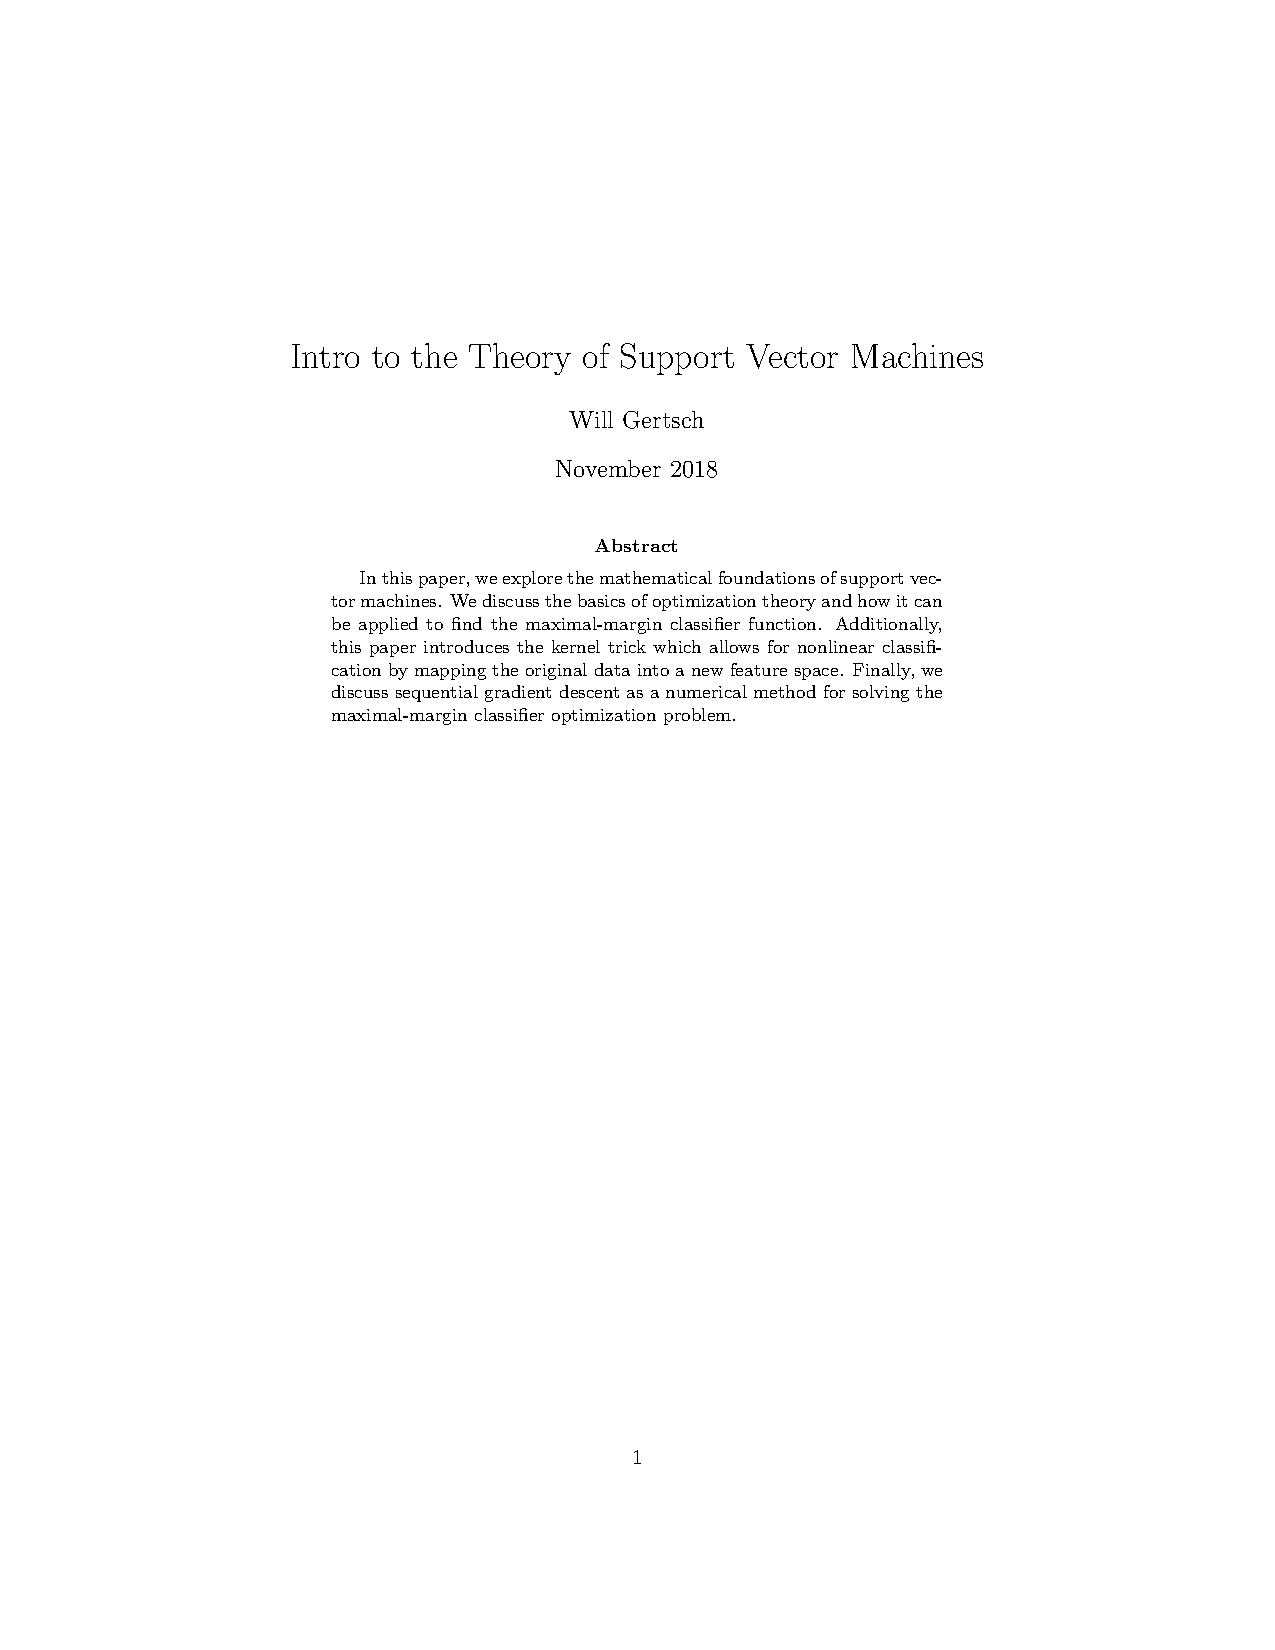
\includegraphics[scale=2]{svm}
\textit{https://commons.wikimedia.org/w/index.php?curid=73710028}
\end{center}

SVMs have many practical applications where it is desired construct a classification model. One such application is identifying the author of document based on the frequency of words. In \textit{The Disputed Federalist Papers: SVM Feature Selection via Concave Minimization}, the author was able to identify Federalist papers of unknown authorship by examining the frequency of certain words in papers where the author is known. Using SVM, he was able to find the separating hyperplane
$$ -0.5368\text{to} - 24.6634\text{upon} - 2.9532\text{would} = -66.6159$$
This model was able to classify the authorship of the disputed papers such that the results agreed with more traditional research on authorship. This example shows the power that SVM has to solve these kinds of classification problems.

\section{Computing the Classification Function}
\subsection{Optimization}
Optimization theory provides a framework for describing problems where it desired to find the maximum or minimum of a function subject to certain constraints. These kind of problems appear often in statistical learning because the training process will involve minimizing the chance that any future data is incorrectly classified. Support vector machines is one such method that can be reduced to an optimization problem.

Before discussing the specific optimization problem in support vector machines, it is important to outline the basics of optimization theory. Firstly, there is a common format for all optimization problems.

\paragraph{Def} The \textit{primal optimization problem} is as follows. Given functions $f$, $g_i$, $i=1,\dots,k$, and $h_i$, $i = 1,\dots,m$, defined on a domain $\Omega \subseteq \mathbb{R}^n$,
$$ minimize \quad f(\mathbf{w}), \mathbf{w} \in \Omega$$
$$ subject\ to \quad g_i(\mathbf{w}) \geq 0, h_i(\mathbf{w}) = 0$$
where $f(\mathbf{w})$ is the \textit{objective function} and the other functions are the \textit{inequality} and \textit{equality} constraints.

Note that this definition provides common terms for a large range of optimization problems, not just minimization problems. All optimization problems can be rephrased in the form of a primal optimization problem. For example, a maximization problem can be rephrased as the negative of a minimization problem.

One possible issue in solving these optimization problems is local extrema. Many methods for solving optimization problems will get "stuck" at a local maximum or minimum. For example, the first derivative test will identify all points where the derivative is zero, whether these points be local or global. To get around this problem, we define a special class of optimization problems.

\paragraph{Def} A real-valued function $f(\mathbf{w})$ is \textit{convex} if $\forall \mathbf{w},\mathbf{u} \in \mathbb{R}^n$ and for $\theta \in (0,1)$,
$$ f(\theta \mathbf{w}+(1-\theta)\mathbf{u}) \leq \theta f(\mathbf{w}) + (1-\theta)f(\mathbf{u})$$
An optimization problem where the objective function and all of the constraint functions are convex is unsurprisingly called a \textit{convex optimization problem}.

Intuitively, a convex function will not have any local extrema.

The primal form is the most basic statement of an optimization problem but it often has the problem where the constraints are difficult handle directly. Therefore, we need to find a way to restate the primal problem in a way that makes the constraints easier to deal with. To do that, we have the following definition.
\paragraph{Def:} Given an optimization problem with objective function $f(\bw)$, inequality constraints $h_i(\bw)$, and equality constraints $g_i(\bw)$, with domain $\Omega \subset \mathbb{R}^n$, we defined the \textit{generalized Lagrangian function} as 
$$ L(\bw, \balpha, \bbeta) = f(\bw) = \sum_{i=1}^k \alpha_i g_i(\bw)+ \sum_{i=1}^m \beta_i h_i(\bw)$$
$$ = f(\bw) + \balpha' \mathbf{g}(\bw)+ \mathbf{\beta}' \mathbf{h}(\bw)$$
The \textit{Lagrangian dual problem} is the following:
$$ maximize \quad \theta(\balpha, \bbeta),$$
$$ subject\ to \quad \balpha \geq \mathbf{0},$$
where $\theta(\balpha, \bbeta) = \inf_{\bw \in \Omega} L(\bw, \balpha, \bbeta)$. The coefficients, $\balpha$ and $\bbeta$, are known as \textit{Lagrange multipliers}.

The advantage of this form of optimization problem is that there is a nice result that uses calculus in order to specify the conditions for an optimal solution. The following theorem is similar to the technique usually taught in multivariable calculus of using Lagrange multipliers to find the extrema of functions. 

\paragraph{Kuhn-Tucker Theorem} Given the usual optimization problem with objective function $f(\bw)$, if $f \in C^1$ and is convex then $\bw^*$ will be the optimal solution given the existence of $\balpha^*$, $\bbeta^*$ such that
$$ \frac{\partial L(\bw^*, \balpha^*, \bbeta^*)}{\partial \bw} = 0, \frac{\partial L(\bw^*, \balpha^*, \bbeta^*)}{\partial \beta} = 0$$
$$ \alpha_i^*g_i(\bw^*) = 0, i = 1, \dots, k$$
$$ g_i(\bw^*) \leq 0, i = 1, \dots, k$$
$$ \alpha_i^* \geq 0, i = 1, \dots, k$$

This set of conditions results in two systems of equations, one for the critical points and one for the constraints. If both the systems are solved simultaneously, then an optimal solution within the feasible region can be computed. In practice, large optimization problems, such as the one in support vector machines, cannot be easily solved by symbolically. Therefore, we must rely on numerical techniques in order to find the desired solution. One such method for solving the systems related the support vector machines will be discussed in section 4.

\subsection{The Max-Margin Classifier}
These optimization techniques are important in the context of statistical learning because the training process often involves minimizing some objective function that directly relates to the accuracy of the model for future data. Optimization theory therefore provides tools for stating statistical learning problems.

Support vector machines is one such method that can be described using optimization theory. There are several ways to model support vector machines, but the simplest is the maximum margin classifier. Simply put, the maximal margin classifier optimization problem computes the separating hyperplane $(\bw,b)$ where $\bw$ is the normal vector and $b$ is the distance from the origin.

\paragraph{Def} Consider a linearly separable training sample
$$ S = ((\mathbf{x}_1,y_1),\dots, (\mathbf{x}_n, y_n))$$
the hyperplane $(\bw, b)$ that solves the optimization problem
$$ minimize_{\bw, b} \quad \langle \bw \cdot \bw \rangle  $$
$$ subject\ to \quad y_i(\langle \bw \cdot \mathbf{x}_i \rangle + b) \geq 1, i = 1, \dots, n$$
is the \textit{maximal margin hyperplane} with margin $\gamma = 1/||\bw||_2$.

Using the Lagrangian duality technique discussed earlier, we can rewrite the optimization problem as the following, 
$$ maximize \quad W(\alpha) = \sum_{i=1}^n \alpha_i - \frac{1}{2}\sum_{i,j=1}^n y_i y_j \alpha_i \alpha_j  \langle \mathbf{x}_i, \mathbf{x}_j \rangle,$$
$$ subject\ to \quad \sum_{i=1}^n y_i \alpha_i = 0,, \alpha_i \geq 0, i=1,\dots,n.$$
Note that $b$ drops out when taking the partial derivatives needed to calculate the Lagrangian. To fix that, we calculate the solution for $b$, $b^*$, by going back to the primal constraints as follows,
    $$ b^* = \frac{\max_{y_i=-1}(\langle \bw^* \cdot \mathbf{x}_i \rangle)+ \min_{y_i=1}(\langle \bw^* \cdot \mathbf{x}_i\rangle)}{2}$$
    
Now, to complete this section, it will be interesting to demonstrate a further result that gives SVM its name. The starting point for deriving the margin, $\gamma = 1/||\bw||_2$, was 
$$ \langle \bw \cdot \mathbf{x}^+ \rangle + b = 1$$
$$ \langle \bw \cdot \mathbf{x}^- \rangle + b = -1$$
where $\mathbf{x}^+$, $\mathbf{x}^-$ are points on the margin above and below the line respectively. Thus $\mathbf{x}^+$, $\mathbf{x}^-$ will be the points that the optimized margin of the hyperplane ends up "touching". Using the Kuhn-Tucker theorem, we get the following information about the optimal solutions $\balpha^*$, $(\bw^*, b^*)$:
$$ \alpha_i^* \left[ y_i(\langle \bw^* \cdot \mathbf{x}_i) \rangle + b^*)-1  \right] = 0, i=1,\dots,n$$
Combining the first equations and the last equation, we see that the term in brackets will be zero if $\mathbf{x}_i$ is one of the points on the margin. Otherwise, $\alpha_i^*$ will need to be zero for the equation to hold. Therefore, we can express the hyperplane using only the vectors that are directly on the margin since these are the only points where $\alpha_i^*$'s will be non-zero. Namely,
$$ f(\mathbf{x}, \balpha^*, b^*) = \sum_{i \in SV} y_i \alpha_i^* \langle \mathbf{x}_i \cdot \mathbf{x} \rangle + b^*$$
The set, SV, is the set of all vectors that directly determine the margin of the separating hyperplane. If $\mathbf{x} \in SV$, then $\mathbf{x}$ is a \textit{support vector}.

The fact that the hyperplane is solely determined by the support vectors allows the same hyperplane to determined only using a subset of the data. This result is useful in reducing classification error. In general, a hyperplane determined by small number of support vectors will have lower classification error than a hyperplane with a large number of support vectors.

\section{Kernel Trick}

\subsection{Non-linear Classification}
Linear support vector machines work well in a wide variety of data but the approach has a few limitations. The main drawback from the basic support vector machine using the maximal-margin classifier is that the resulting classification function is linear. That means that this basic form of SVM can only perform linear classification. If the data is not \textit{linear separable}, then the maximal-margin classifier will be unable to correctly classify all of the training data. 

\vspace{100pt}

\begin{center}
\textbf{Figure 2: Non-linearly Separable Data}
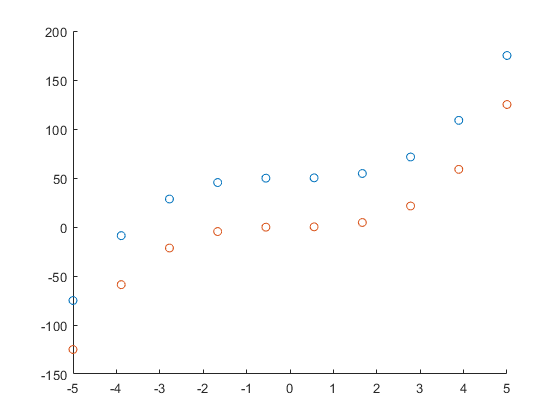
\includegraphics[scale=0.5]{nonlinearex}
\end{center}

Figure 2 is an example of data that cannot be linearly separated, i.e. there is no plane that can be drawn such that all the blue points are on one side of the line and all the red points are on the other. However, there is clearly a way to classify the data. The plot was created by taking 10 values of $f(x) = x^3$ and $g(x) = x^3 +50$ so a good classification function in this case might be $h(x) = x^3 +25$. 

Therefore, there is a need to classify nonlinear data in a way that the basic SVM algorithm cannot. However, there is a way to extend SVM in order to handle nonlinear classification functions. The beauty of the SVM approach is that extending the maximal-margin classifier to be able handle nonlinear data is simple.

\subsection{The Kernel Trick}
The way in which SVM supports nonlinear classification is by projecting the input data into a new feature space by using a special function. In general, we want
$$ \mathbf{x} = (x_1, \dots, x_n) \mapsto \bphi(\mathbf{x}) = (\phi_1(\mathbf{x}), \dots, \phi_d(\bx))$$
with ideally $d < n$ such that we reduce the number of dimensions of the feature space. The goal is to generate a feature space where the images of points can be linearly separated.

\begin{samepage}
\begin{center}

\textbf{Figure 3: Kernel Mapping to New Feature Space}
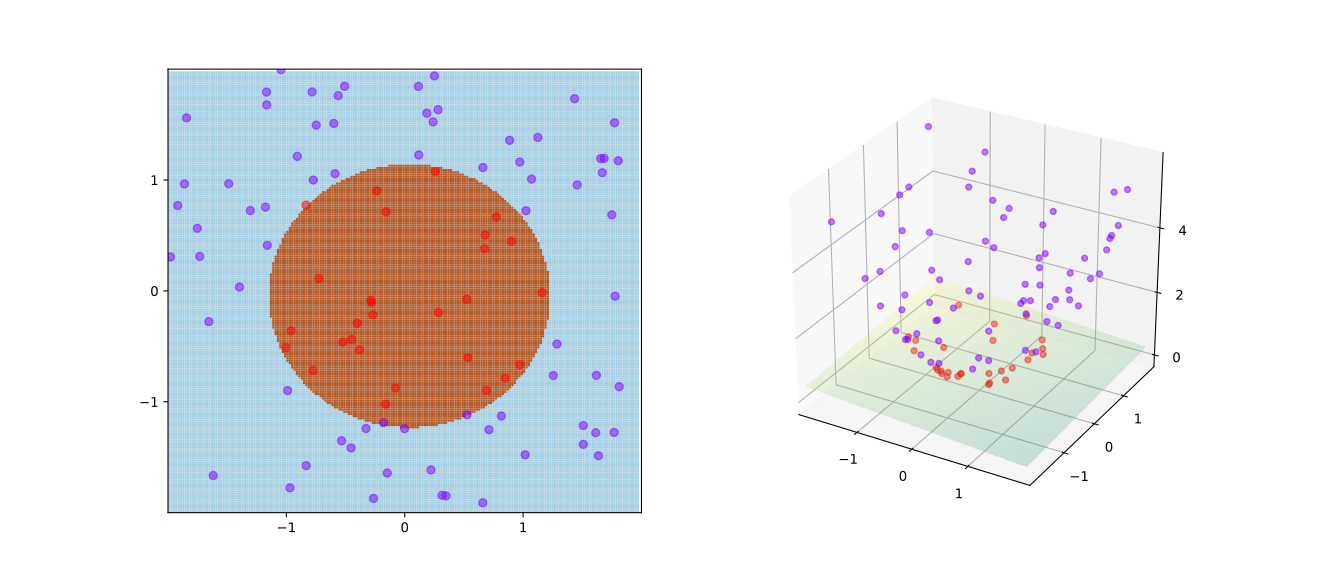
\includegraphics[scale=0.30]{kerneltrick}
\nopagebreak
\textit{https://commons.wikimedia.org/w/index.php?curid=60458994}
\end{center}
\end{samepage}

Figure 2 gives an example where a 2-dimensional space is mapped to 3-dimensional space where a linear classification is now possible. The green hyperplane in second image is result of running SVM on the feature space and the orange circle is the corresponding classifier in the original space.

This mapping is achieved by replacing the inner product in the maximal-margin classifier with a \textit{kernel function}, i.e.
$$ f(\mathbf{x}, \balpha^*, b^*) = \sum_{i \in SV} y_i \alpha_i^* \langle \mathbf{x}_i \cdot \mathbf{x} \rangle + b^*$$
becomes
$$ f(\mathbf{x}, \balpha^*, b^*) = \sum_{i \in SV} y_i \alpha_i^* K(\mathbf{x}_i \cdot \mathbf{x}) + b^*$$
The kernel function is a generalization of inner product from the input space. This substitution works since the data vectors, the $\mathbf{x}$'s, are not found anywhere else in the function. In practice, kernel functions are chosen based on the given data that needs to be classified. Because of this, there are wide variety of possible kernel functions that can be used in SVM, ranging from polynomials, to Gaussian functions and wavelets. Discussion of the official definition and necessary conditions for a mapping to be  a kernel function is beyond the scope of this paper. 

\subsection{Polynomial Kernels}
One of the simplest kernels is the polynomial kernel. This kernel replaces the dot product with a polynomial based on the vector components. For example, a 2-dimensional polynomial kernel is derived as follows
\begin{align*}
 K(\mathbf{x}, \mathbf{z}) &= (\langle \mathbf{x} \cdot \mathbf{z} \rangle+c)^2\\
 &= \left( \sum_{i=1}^n x_i z_i \right)^2+2c\left( \sum_{i=1}^n x_i z_i \right)+c^2
\end{align*}
by "foiling" the inner-product and the constant. Similarly, we can construct a polynomial kernel of dimension $d$ by expanding
$$ K(\mathbf{x}, \mathbf{z}) = (\langle \mathbf{x} \cdot \mathbf{z} \rangle+c)^d $$
The resulting variables in the feature space will be monomials of degree less than or equal to $d$. For example, a 2-dimensional case with a degree 2 polynomial will be
$$ (x_1, x_2) \mapsto \bphi(x_1, x_2) = (x_1^2,x_2^2, x_1x_2)$$

The choice of $d$ will depend on original data. For instance, the data in Figure 2 can be separated by letting $d=3$ to let SVM generate a degree polynomial such as $h(x) = x^3+25$. 

\section{Computational Methods}
\subsection{Motivation}
The previous sections were primarily concerned with stating the optimization problem that leads to the separating hyperplane classification function. At its core, the maximal-margin optimization is just a Lagrange multipliers problem. At small scales, it is possible to solve for the Lagrange multipliers by hand using symbolic manipulation. This approach is simply not possible in the case of SVM since the objective function is very complex and there can be thousands of multipliers to solve for. These factors require numerical methods in order to solve the SVM problem.

There are a few methods that can be used to numerically solve the maximal margin optimization problem. One of the more sophisticated methods is Sequential Minimal Optimization, which takes advantage of the specifics of the SVM problem to efficiently find the solution. However, the theory used in SMO goes beyond the scope of this paper. Instead, we will discuss a simpler algorithm for solving the maximal margin problem.

\subsection{Sequential Gradient Ascent}
This method is the naive solution in that it does not consider the structure of the problem to compute the solution. Instead, gradient ascent needs only the objective function and the constraints. As the name suggests, gradient descent relies heavily on the gradient of $W(\balpha)$. The $i$th component of $\nabla W(\balpha)$ is 
$$ \frac{\partial W(\balpha)}{\partial \alpha_i} = 1 - y_i \sum_{j=1}^n \alpha_i y_i K(\mathbf{x}_i, \mathbf{j} ) $$
The method, given an initial starting point, $\balpha_t$, computes $\balpha_{t+1}$ by computing the gradient at $\balpha_t$ and taking a step of size $h$ in the direction of the gradient. This amounts to finding direction in which the ascent is the steepest and then moving in that direction. Additionally, the method must check every step to see if the constraints are still satisfied.

Sequential gradient ascent does this by stepping a single component at a time, i.e.
$$ \alpha_i \leftarrow  \alpha_i +h \frac{\partial W(\balpha)}{\partial \alpha_i}$$
Therefore, the sequential method has the advantage that it reduces a multidimensional problem into 1-dimensional steps. Once each component has been updated, the algorithm checks to see if the current step is close enough to optimal solution by checking one of several stopping criteria from the underlying optimization theory.  

\section{Conclusion}
This has been only a brief introduction to the theory of support vector machines. SVMs are powerful in that they provide a general framework for solving a wide range optimization problems. Besides linear and nonlinear binary classification with simple kernels, SVMs can also be used with more complicated kernels, be stacked in layers for n-classification problems, and even be modified to generate  regression models. This flexibility makes SVM a strong alternative to other machine learning methods such as neural networks.

\pagebreak
\section{Appendix}
MATLAB implementation is forthcoming.

\pagebreak
\section{References}

\begin{flushleft}
Cristianini, N., Shawe-Taylor, J., (2000). \textit{An Introduction to Support Vector Machines and other kernel-based learning methods}  Cambridge University Press.
\end{flushleft}

\begin{flushleft}
Wikipedia contributors, "Support vector machine," Wikipedia, \textit{The Free Encyclopedia},  \href{https://en.wikipedia.org/w/index.php?title=Support_vector_machine&oldid=866892968}{URL} (accessed November 17, 2018).
\end{flushleft}


\end{document}
